\documentclass[a4paper, 11pt]{article}
\usepackage[utf8]{inputenc}
\usepackage[total={17cm, 24cm}, top=3cm, left=2cm]{geometry}
\usepackage{times}
\usepackage[czech]{babel}
\usepackage{hyperref}
\usepackage{graphicx}
\usepackage{tabu,array,multirow}
\usepackage{amsmath}
\usepackage[czech,linesnumbered,lined,commentsnumbered,ruled]{algorithm2e}
\usepackage{algorithmic}
\usepackage{xcolor, picture}
\usepackage{pdflscape}

\renewcommand{\algorithmicrequire}{\textbf{Input:}}
\renewcommand{\algorithmicensure}{\textbf{Output:}}
\newcommand{\thedate}{\today}

\date{March 2019}

\begin{document}
\begin{titlepage}
\begin{center}
\Huge\textsc{Vysoké učení technickév~Brně\\
\huge{Fakulta informačních technologií}}\\
\vspace{\stretch{0.382}}
\LARGE{Typografie a publikování\,--\,3. projekt}\\
\Huge Tabulky a obrázky\\
\vspace{\stretch{0.618}}
\end{center}
{\Large 28. března 2019 \hfill Boris Burkalo}
\end{titlepage}


\section{Úvodní strana}\label{1}
Název práce umístěte do zlatého řezu a nezapomeňte uvést dnešní datum a vaše jméno a příjmení.

\section{Tabulky}\label{2}
Pro sázení tabulek můžeme použít buď prostředí\texttt{ tabbing }nebo prostředí\texttt{ tabular}.

\subsection{Prostředí \texttt{tabbing}}
Při použití\texttt{ tabbing } vypadá tabulka následovně:
\begin{tabbing}
ovoce melouny ~~~~\= cena ~~~~
\= množství \kill
\bfseries Ovoce \>
\bfseries Cena \>
\bfseries Množství \\
Jablka \> 25,90 \> 3 kg \\
Hrušky \> 27,40 \> 2,5 kg \\
Vodní melouny \> 35,- \> 1 kus\\
\end{tabbing}
Toto prostředí se dá také použít pro sázení algoritmů, ovšem vhodnější je použít
prostředí\texttt{ algorithm }nebo\texttt{ algorithm2e }(viz sekce \ref{3}).

\subsection{Prostředí \texttt{tubular}}
Další možností, jak vytvořit tabulku, je použít prostředí\texttt{ tabular}. Tabulky pak
budou vypadat takto\footnote{Kdyby byl problém s\texttt{ cline }, zkuste se podívat třeba sem: \hyperlink{http://www.abclinuxu.cz/tex/poradna/show/325037}{http://www.abclinuxu.cz/tex/poradna/show/325037}.}: \\
\begin{table}[h]
\begin{center}
\catcode`\-=12
 \begin{tabular}{|c|c|c|c|c|}
 \hline
 & \multicolumn{2}{c|}{\textbf{Cena}} \\\cline{2-3}
\textbf{Měna} & \textbf{nákup} & \textbf{prodej} \\
 \hline
EUR & 25,615 & 27,20 \\
GBP & 29,899 & 31,80 \\
USD & 22,571 & 25,51 \\
\hline
 \end{tabular}
\caption{Tabulka kurzů k dnešnímu dni}
\label{tab1}
\end{center}
\end{table}

\begin{table}[h]
\begin{tabular}{|c|c|c|c|c}
\hline
    $A$ & $\neg A$ \\\hline
    \textbf{P} & N \\\hline
    \textbf{O} & O \\\hline
    \textbf{X} & X \\\hline
    \textbf{N} & P \\\hline

\end{tabular}
\catcode`\-=12
\begin{tabular}{|c|c|c|c|c|c|}
\hline
    \multicolumn{2}{|c|}{\multirow{2}{*}{$A \land B$}} & \multicolumn{4}{c|}{$B$} \\\cline{3-6}
     \multicolumn{2}{|c|}{} & \textbf{P} & \textbf{O} & \textbf{X} & \textbf{N} \\\hline
    \multirow{4}{*}{$A$} & \textbf{P} & P & O & X & N\\\cline{2-6}
    & \textbf{O} & O & O & N & N\\\cline{2-6}
    & \textbf{X} & X & N & X & N\\\cline{2-6}
    & \textbf{N} & N & N & N & N\\\hline

\end{tabular}
\catcode`\-=12
\begin{tabular}{|c|c|c|c|c|c|}
\hline
    \multicolumn{2}{|c|}{\multirow{2}{*}{$A \lor B$}} & \multicolumn{4}{c|}{$B$} \\\cline{3-6}
     \multicolumn{2}{|c|}{} & \textbf{P} & \textbf{O} & \textbf{X} & \textbf{N} \\\hline
    \multirow{4}{*}{$A$} & \textbf{P} & P & P & P & P\\\cline{2-6}
    & \textbf{O} & P & O & P & O\\\cline{2-6}
    & \textbf{X} & P & P & X & X\\\cline{2-6}
    & \textbf{N} & P & O & X & N\\\hline

\end{tabular}
\catcode`\-=12
\begin{tabular}{|c|c|c|c|c|c|}
\hline
    \multicolumn{2}{|c|}{\multirow{2}{*}{$A \to B$}} & \multicolumn{4}{c|}{$B$} \\\cline{3-6}
     \multicolumn{2}{|c|}{} & \textbf{P} & \textbf{O} & \textbf{X} & \textbf{N} \\\hline
    \multirow{4}{*}{$A$} & \textbf{P} & P & O & X & N\\\cline{2-6}
    & \textbf{O} & P & O & P & O\\\cline{2-6}
    & \textbf{X} & P & P & X & X\\\cline{2-6}
    & \textbf{N} & P & P & P & P\\\hline
\end{tabular}
\caption{Protože Kleeneho trojhodnotová logika už je \uv{zastaralá}, uvádíme si zde příklad čtyřhodnotové logiky}
\label{tab2}
\end{table}

\section{Algoritmy}\label{3}

Pokud budeme chtít vysázet algoritmus, můžeme použít prostředí \texttt{ algorithm\footnote{Pro nápovědu, jak zacházet s prostředím \texttt{algorithm}, můžeme zkusit tuhle stránku: \\
\hyperlink{http://ftp.cstug.cz/pub/tex/CTAN/macros/latex/contrib/algorithms/algorithms.pdf}{http://ftp.cstug.cz/pub/tex/CTAN/macros/latex/contrib/algorithms/algorithms.pdf.} }} nebo \texttt{ algorithm2e\footnote{Pro \texttt{ algorithm2e} zase tuhle: \hyperlink{http://ftp.cstug.cz/pub/tex/CTAN/macros/latex/contrib/algorithm2e/algorithm2e.pdf}{http://ftp.cstug.cz/pub/tex/CTAN/macros/latex/contrib/algorithm2e/algorithm2e.pdf.} }}.
Příklad použití prostředí \texttt{ algorithm2e } viz Algoritmus \ref{algoritmus1}.

\begin{algorithm}
    \begin{algorithmic}[1]
        \REQUIRE{($X_{t-1}, u_t, z_t$)}
        \ENSURE {$X_t$}
        \STATE $\overline{X_t} = X_t = 0$
        \FOR{$k = 1\ \text{to}\ M$}
        \STATE $x^{[k]} = sample\_motion\_model(u_t,x^{[k]}_{t-1})$
        \STATE $w^{k}_t = measurement\_model(z_t,x_t^{[k]}$
        \STATE $m^{k}_t = updated\_occupancy\_grid(z_t,x_t^{[k]},m_{t-1}^{[k]})$
        \STATE $\overline{X_t} = \overline{X_t} + \langle x_x^{[m]},w_t^{[m]}$
        \ENDFOR
        \FOR{$k = 1\ \text{to}\ M$}
        \STATE draw $i$ with probability $\approx w_i^{[t]}$
        \STATE add $\langle x_x^{[k]},m_t^{[k]}\rangle$ to $X_t$
        \ENDFOR
        \RETURN $X_t$
    \end{algorithmic}
    \caption{\textsc{fast}SLAM}
    \label{algoritmus1}
\end{algorithm}


\section{Obrázky}\label{4}
Do našich článků můžeme samozřejmě vkládat obrázky. Pokud je obrázkem fotografie,
můžeme klidně použít bitmapový soubor. Pokud by to ale mělo být nějaké schéma nebo
něco podobného, je dobrým zvykem takovýto obrázek vytvořit vektorově.

\begin{figure}[h]
\centering
\scalebox{0.4}{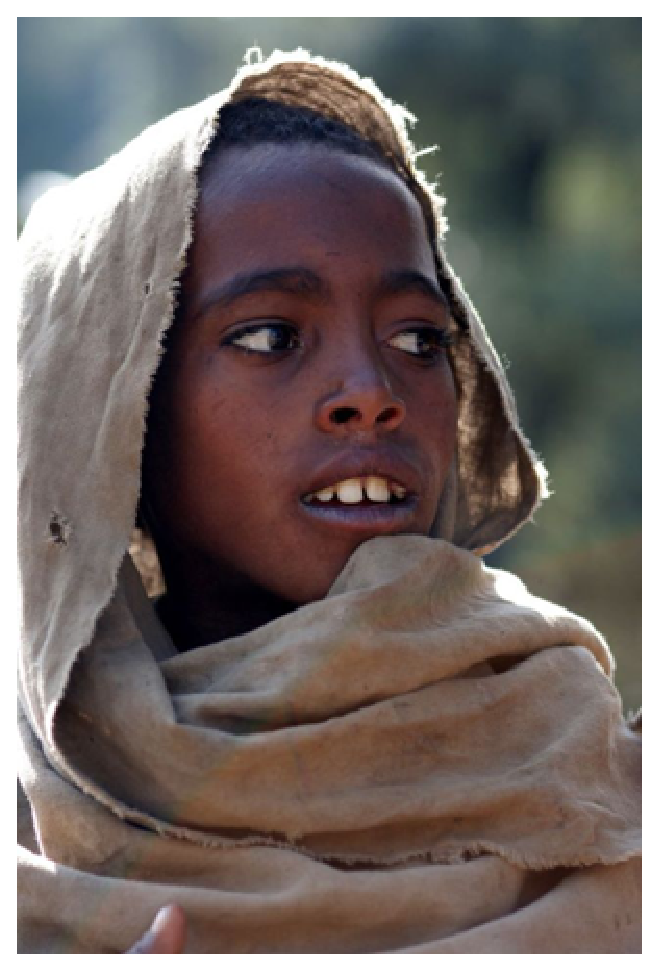
\includegraphics{etiopan.eps}
\reflectbox{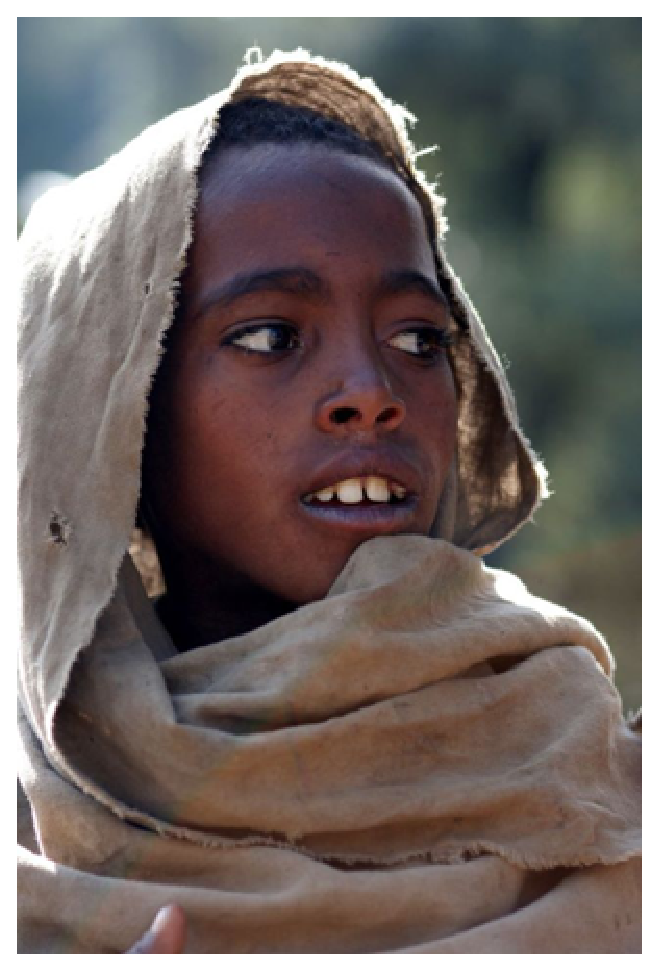
\includegraphics{etiopan.eps}} }
\caption{Malý Etiopánek a jeho bratříček}
\label{obrazek1}
\end{figure}

\pagebreak

Rozdíl mezi vektorovým $\ldots$
\begin{figure}[h]
    \centering
    \scalebox{0.4}{
\includegraphics{oniisan.eps}}
    \caption{Vektorový obrázek}
    \label{obrazek2}
\end{figure}
\\
$\ldots$ a bitmapovým obrázkem

\begin{figure}[h]
    \centering
    \scalebox{0.6}{
\includegraphics{oniisan2.eps}}
    \caption{Bitmapový obrázek}
    \label{obrazek3}
\end{figure}
se projeví například při zvětšení.

Odkazy (nejen ty) na obrázky \ref{obrazek1}, \ref{obrazek2} a \ref{obrazek3}, na
tabulky \ref{tab1} a \ref{tab2} a také na Algoritmus \ref{algoritmus1} jsou udělány pomocí
křížových odkazů. Pak je ovšem potřeba zdrojový soubor přeložit dvakrát.

Vektorové obrázky lze vytvořit i přímo v \LaTeX u, například pomocí prostředí
\texttt{ picture}.


\begin{landscape}
\begin{figure}
\setlength{\unitlength}{4pt}
    \begin{center}
        \begin{picture}(150, 100)(0,0)
        \setlength\fboxsep{0pt}
        \put(0,0){\framebox(150,100)}

        %%%1st house (My)
        \put(50,20){\framebox(50, 65)}
        \put(57,70){\framebox(15, 7.5)}
        \put(64.5,64){\framebox(7.5, 5)}
        \put(64.5,64){\framebox(7.5, 13.5)}
        \put(79,70){\framebox(15, 7.5)}
        \put(57,50){\framebox(15, 7.5)}
        \put(64.5,44){\framebox(7.5, 5)}
        \put(64.5,44){\framebox(7.5, 13.5)}
        \put(79,50){\framebox(15, 7.5)}
        \put(77,20){\framebox(19, 15)}
        \put(77,20){\framebox(19, 5)}
        \put(77,20){\framebox(19, 10)}
        \put(77,20){\framebox(19, 15)}
        \put(76,20){\framebox(21, 16)}
        \put(56.5,20){\framebox(14, 15)}
        \put(56.5,20){\framebox(4, 15)}
        \put(57.5,22){\framebox(2, 11)}
        \put(63.5,22){\framebox(4, 11)}
        \put(70.5,20){\framebox(4, 15)}
        \put(71.5,22){\framebox(2, 11)}
        \put(68.5,28){\line(1,0){2}}
        \put(0,20){\line(1,0){150}}

        %%%Neighbours house
        \put(0,20){\framebox(46, 65)}
        \put(3,70){\framebox(15, 7.5)}
        \put(10.5,64){\framebox(7.5, 5)}
        \put(10.5,64){\framebox(7.5, 13.5)}
        \put(25,70){\framebox(15, 7.5)}
        \put(3,50){\framebox(15, 7.5)}
        \put(10.5,44){\framebox(7.5, 5)}
        \put(10.5,44){\framebox(7.5, 13.5)}
        \put(25,50){\framebox(15, 7.5)}
        \put(23,20){\framebox(19, 15)}
        \put(23,20){\framebox(19, 5)}
        \put(23,20){\framebox(19, 10)}
        \put(23,20){\framebox(19, 15)}
        \put(22,20){\framebox(21, 16)}
        \put(2.5,20){\framebox(14, 15)}
        \put(2.5,20){\framebox(4, 15)}
        \put(3.5,22){\framebox(2, 11)}
        \put(9.5,22){\framebox(4, 11)}
        \put(16.5,20){\framebox(4, 15)}
        \put(17.5,22){\framebox(2, 11)}
        \put(14.5,28){\line(1,0){2}}

        %%%3rdHOUSE
        \put(104,20){\framebox(46, 65)}
        \put(111,70){\framebox(15, 7.5)}
        \put(118.5,64){\framebox(7.5, 5)}
        \put(118.5,64){\framebox(7.5, 13.5)}
        \put(133,70){\framebox(15, 7.5)}
        \put(111,50){\framebox(15, 7.5)}
        \put(118.5,44){\framebox(7.5, 5)}
        \put(118.5,44){\framebox(7.5, 13.5)}
        \put(133,50){\framebox(15, 7.5)}
        \put(131,20){\framebox(19, 15)}
        \put(131,20){\framebox(19, 5)}
        \put(131,20){\framebox(19, 10)}
        \put(131,20){\framebox(19, 15)}
        \put(130,20){\framebox(20, 16)}
        \put(110.5,20){\framebox(14, 15)}
        \put(110.5,20){\framebox(4, 15)}
        \put(111.5,22){\framebox(2, 11)}
        \put(117.5,22){\framebox(4, 11)}
        \put(124.5,20){\framebox(4, 15)}
        \put(125.5,22){\framebox(2, 11)}
        \put(122.5,28){\line(1,0){2}}




        \linethickness{1.5pt}
        %%%MY HOUSE
        \put(51,63){\framebox(48, 7)}
        \put(51,43){\framebox(48, 7)}
        \put(0,20){\line(1,0){150}}
        %%%N.house
        \put(0,63){\framebox(45, 7)}
        \put(0,43){\framebox(45, 7)}
        %%3rd HOUSE
        \put(105,63){\framebox(45, 7)}
        \put(105,43){\framebox(45, 7)}


        \linethickness{1pt}
        %%MY HOUSE
        \put(95,20){\line(-1,-6){3.36}}
        \put(88,20){\line(-1,-6){3.36}}
        \put(78,20){\line(-1,-6){3.35}}
        \put(85,20){\line(-1,-6){3.35}}
        \put(60,20){\line(-1,-6){3.35}}
        \put(71,20){\line(-1,-6){3.35}}
        \put(50,82){\framebox(50, 3)}
        \put(50,20){\framebox(1, 65)}
        \put(99,20){\framebox(1, 65)}
        \put(46,20){\colorbox{black!4}{\framebox(4,65){}}}
        \put(100,20){\colorbox{black!4}{\framebox(4,65){}}}

        %%N.house
        \put(45,20){\framebox(1, 65)}
        \put(0,82){\framebox(46, 3)}
        %%3rd HOUSE
        \put(100,82){\framebox(50, 3)}

        %%3rd HOUSE
        \put(104,20){\framebox(1, 65)}

        \put(137.5, 92.5){\circle{20}}


        \end{picture}
        \end{center}
        \caption{Vektorový obrázek mého (prostřední) řadového domu.}
        \label{obrazek4}
    \end{figure}
\end{landscape}


\end{document}
